\documentclass[border=4pt]{standalone}
\usepackage{tikz}
\usetikzlibrary{arrows.meta,calc,shapes.misc}

\begin{document}
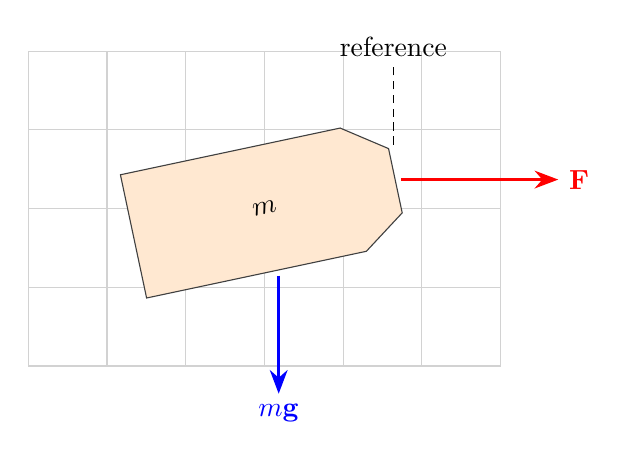
\begin{tikzpicture}[>=Stealth]
  \draw[gray!35] (-3,-2) grid[step=1cm] (3,2);
  \node[shape=chamfered rectangle,rotate=12,draw=black!75,fill=orange!18,
    chamfered rectangle angle=55,chamfered rectangle sep=3mm,
    chamfered rectangle corners={north east,south east},
    minimum width=34mm,minimum height=16mm,outer sep=2pt] (body) at (0,0) {$m$};

  \draw[-{Stealth[length=3mm]},red,line width=1.1pt]
    (body.east) -- ++(0:20mm) node[right] {$\mathbf F$};
  \draw[-{Stealth[length=3mm]},blue,line width=1.1pt]
    (body.south) -- ++(-90:15mm) node[below] {$m\mathbf g$};
  \draw[densely dashed] (body.before north east) -- ++(90:10mm);
  \node[above] at ($(body.before north east)+(0,10mm)$) {reference};
\end{tikzpicture}
\end{document}
